\documentclass[pdf, hyperref={unicode}, aspectratio=169]{beamer}

\usepackage{styles}

\usepackage{qrcode}
\usepackage{tikz}
\usepackage{xifthen}
\usepackage[export]{adjustbox}

\usetikzlibrary{arrows.meta, positioning, fit, backgrounds, calc, shapes.geometric}

\title{Предотвращение взаимоблокировок автономных агентов методами централизованного планирования}

\subtitle{Выпускная квалификационная работа студента СпецВО}

\pdfstringdefDisableCommands{
  \def\\{}
  \def\,{}
  \def\textbf#1{<#1>}
}

\author[Бирюков Виктор Владимирович]
{
  \textbf{Студент группы М8О-208СВ-24:} Бирюков Виктор Владимирович\\
  \ \textbf{Научный руководитель:} д.т.н., доц., проф. каф. 806 В.\,А.\,Судаков
}

\institute[Московский авиационный институт]
{
  Московский авиационный институт (национальный исследовательский университет)\\
  Институт № 8 «Компьютерные науки и прикладная математика»\\
  Кафедра № 806 «Вычислительная математика и программирование» 
}

\date{Москва --- \the\year}

\logo{\includegraphics[height=1cm]{template/img/mai}}

\newcommand{\mycolorbar}[6]% height,width,colors,label min,label max,label step
{   \begin{tikzpicture}
        \foreach \x [count=\c] in {#3}{ \xdef\numcolo{\c}}
        \pgfmathsetmacro{\pieceheight}{#1/(\numcolo-1)}
        \xdef\lowcolo{}
        \foreach \x [count=\c] in {#3}
        {   \ifthenelse{\c = 1}
            {}
            {   \fill[bottom color=\lowcolo,top color=\x] (0,{(\c-2)*\pieceheight}) rectangle (#2,{(\c-1)*\pieceheight});
            }
            \xdef\lowcolo{\x}
        }
        \draw (0,0) rectangle (#2,#1);
        \pgfmathsetmacro{\secondlabel}{#4+#6}
        \pgfmathsetmacro{\lastlabel}{#5+0.01}
        \pgfkeys{/pgf/number format/.cd,fixed,precision=2}
        \foreach \x in {#4,\secondlabel,...,\lastlabel}
        { \draw (#2,{(\x-#4)/(#5-#4)*#1}) -- ++ (0.05,0) node[right] {\pgfmathprintnumber{\x}};
        }
    \end{tikzpicture}
}

\graphicspath{{./img}, {../report/img/}}

\begin{document}

\frame{\titlepage}

\begin{frame}
\frametitle{Актуальность темы}

\begin{figure}
\textit{график с ростом объема автономного транспорта}
\end{figure}

\note{
Актуальность работы связана с увеличением использования автономного транспорта разных видов...
Сфокусируемся на мелком автономном транспорте
}
\end{frame}


\begin{frame}
\frametitle{Актуальность работы}

\begin{figure}
\textit{график с бенчмарками локального планирования ???}
\end{figure}

\note{
при управлении автономными роботами возникает две задачи планирования
это задача локального планирования и задача глобального планирования
но существуют ситуации в которых локальное планирование может не справляется
и необходимо внешнее вмешательство
на практике оно часто осуществляется ручным удаленным управлением
но можно использовать автоматизированные системы глобального управления
}	
\end{frame}


\begin{frame}
\frametitle{Цель и задача работы}

\textbf{Цель работы} --- разработать методы локального разрешения
конфликтов для глобального управления автономными агентами 
на графе дорожной сети с узкими местами и сопоставить их с классическими
методами многоагентного планирования в задаче предотвращения взаимоблокировок.

\textbf{Задачи:}
\begin{itemize}
    \item формализация задачи и определение метрик качества;
    \item анализ существующих методов многоагентного планирования;  
    \item разработка альтернативные методы управления;
    \item разработка программной среда симуляции и подготовка набора
          тестовых графов;
     \item проведение сравнительный эксперимента.
\end{itemize}
\end{frame}


\begin{frame}
\frametitle{Постановка задачи}

\textbf{Дано:}
\begin{itemize}
	\item Исходные данные
	\item Требования и условия
	\item Ограничения и допущения
	\item Требования к железу, ОС и сетевому окружению
	\item …
\end{itemize}
\end{frame}


\begin{frame}
\frametitle{Многоагентное планирование}

\end{frame}


\begin{frame}
\frametitle{Методы разрешения конфликтов}

\begin{figure}

\includegraphics[height=0.75\textheight]{reverse/frame_0007}

\includegraphics[height=0.75\textheight]{reverse/frame_0055}

\includegraphics[height=0.75\textheight]{reverse/frame_0100}

\includegraphics[height=0.75\textheight]{reverse/frame_0180}
\hfill

\includegraphics[height=0.75\textheight]{semaphore/frame_0007}

\includegraphics[height=0.75\textheight]{semaphore/frame_0055}

\includegraphics[height=0.75\textheight]{semaphore/frame_0100}

\includegraphics[height=0.75\textheight]{semaphore/frame_0140}
\end{figure}

\end{frame}


\begin{frame}
\frametitle{Адаптивное планирование}

\begin{figure}

\includegraphics[height=0.7\textheight]{adaptive/frame_0000}

\includegraphics[height=0.7\textheight]{adaptive/frame_0055}

\includegraphics[height=0.7\textheight]{adaptive/frame_0100}

\includegraphics[height=0.7\textheight]{adaptive/frame_0235}

\includegraphics[height=0.7\textheight]{adaptive/frame_0280}
\hspace{0.5cm}
\mycolorbar{5}{0.4}{red, yellow, green}{0.0}{2.2}{1.1}
\end{figure}

\vfill

\begin{figure}
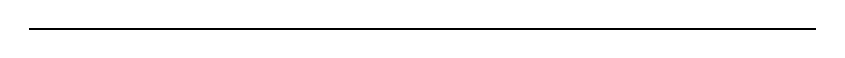
\begin{tikzpicture}
\draw[thick] (0, 0) -- (10, 0);
\end{tikzpicture}
\end{figure}

\end{frame}


\begin{frame}
\frametitle{Архитектура решения}
\framesubtitle{Симулятор}

\begin{figure}
\begin{tikzpicture}[
    scale=0.7,
    font=\small,
    box/.style={draw, rounded corners=2pt, align=center,
                minimum height=10mm, minimum width=30mm, inner sep=3pt},
    core/.style={box, fill=black!5},
    plug/.style={box, dashed},
    io/.style={box, fill=black!2},
    flow/.style={-{Latex[length=2mm]}, thick},
    dep/.style={-{Latex[length=2mm]}, dashed, gray},
    lbl/.style={font=\tiny, inner sep=1pt, fill=white},
]
    % --- Nodes placed on an explicit grid for orthogonal routing ---
    \node[io]   (graph)  at ( 0   ,  5.4) {Граф\\\scriptsize дорожной сети};

    \node[plug] (router) at (-5.6 ,  3.0) {Планировщик\\\scriptsize маршрутов};
    \node[core] (disp)   at ( 0   ,  3.0) {Диспетчер\\\scriptsize заказов};
    \node[plug] (res)    at ( 5.6 ,  3.0) {Разрешение\\\scriptsize конфликтов};

    \node[core] (sim)    at (-2.8 ,  0.6) {Цикл симуляции};
    \node[core] (agent)  at ( 2.8 ,  0.6) {Агенты};

    \node[io]   (stats)  at (-2.8 , -2.4) {Сбор\\\scriptsize метрик};
    \node[io]   (vis)    at ( 2.8 , -2.4) {Визуализация};

    % --- Control / state flow inside the core (solid) ---
    \draw[flow] (disp.west)   -- node[lbl, below]{запрос маршрута}    (router.east);
    \draw[flow] (disp.south)  -- node[lbl, right]{выдача заказов}     (sim.north);
    \draw[flow] (res.south)   -- node[lbl, right]{коррекция}          (agent.north);
    \draw[flow] (sim.east)    -- node[lbl, align=center, fill opacity=0.0, text opacity=1.0]{обновление\\позиции} (agent.west);

    % --- Graph data dependencies (dashed) ---
    \draw[dep] (router.north) -- (router.north |- graph.south) -- (graph.south west);
    \draw[dep] (disp.north)   -- (graph.south);
    \draw[dep] (res.north)    -- (res.north |- graph.south) -- (graph.south east);
    
    % --- Statistics inputs (dashed), each on its own lane ---
    \draw[dep] (sim.south) -- (stats.north);
    
    % --- Visualizer input from agents (dashed) ---
    \draw[dep] (agent.south) -- (vis.north);
    \draw[dep] (graph.east) -- ++(7.0,0) |- (vis.east);

    \begin{scope}[on background layer]
        \node[draw, dotted, rounded corners,
              fit=(router) (disp) (res) (sim) (agent),
              inner sep=4mm,
              label={[font=\footnotesize]below:Ядро симулятора}] {};
    \end{scope}
\end{tikzpicture}
\caption{Структура симулятора и взаимодействие основных компонентов.}
\end{figure}
\end{frame}


\begin{frame}
\frametitle{Исходные данные}

В качестве источника данных использовались фрагменты карты OpenStreetMap

\begin{figure}
\hfill

\includegraphics[height=0.75\textheight, valign=c]{medium_graph}
\hfill

\includegraphics[width=0.75\textheight, valign=c, angle=90, origin=c]{large_graph}
\hfill
\end{figure}

\end{frame}


\begin{frame}
\frametitle{Результаты}

Скрины/Формат вывода данных
\end{frame}


\begin{frame}
\frametitle{Оценка результата}

Перечень ключевых характеристик функционирования разработки
\end{frame}


\begin{frame}
\frametitle{Описание программной разработки}

QR-код ссылки, где выложен код

\begin{figure}
\qrcode[height=0.6\textheight]{https://github.com/iktovr/master-diploma}
\end{figure}
\end{frame}

\begin{frame}
\end{frame}

\end{document}
